
\newpage

\section{File inclusion}

De nombreux langages de programmation permettent d'inclure des portions de code contenues dans d'autres fichiers que celui en cours d'exécution. Le mécanisme mis à disposition permet de recopier dans le script principal le code contenu dans un autre fichier. Cette procédure est transparente à l'œil de l'utilisateur et peut-être très avantageuse pour le développeur d'un site internet.

\begin{figure}[!h]
\begin{center}

\label{inclusion}
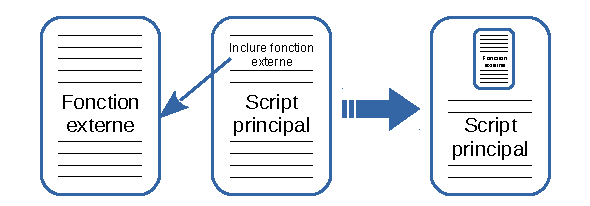
\includegraphics[scale=1.2]{images/include.pdf}

\caption{Mécanisme d'inclusion d'un fichier}

\end{center}
\end{figure}

En effet, inclure du code contenu dans un autre fichier permet, entre autre, les deux utilisations suivantes :
\begin{itemize}
\item inclure des portions de code différentes en fonction de choix de l'utilisateur ou de l'environnement de ce dernier;
\item inclure des portions de code utilisées dans plusieurs scripts (par exemple une fonction de connexion à une base de données) afin de ne pas avoir à recopier les mêmes lignes à différents endroits et de ne modifier qu'un seul fichier en cas de modification de la fonction.
\end{itemize}





\subsection{Description de la vulnérabilité}

La principale vulnérabilité connue dans le mécanisme que nous venons d'expliciter intervient lorsque l'inclusion d'un script est gérée par une variable pouvant être contrôlée par un attaquant. On se retrouve alors plutôt dans le premier cas d'utilisation indiqué, c'est à dire inclure des portions de code différentes en fonction de choix de l'utilisateur ou de l'environnement de ce dernier. En effet, dans le second cas d'utilisation, l'inclusion du fichier est généralement écrite "en dur" dans le script principal et ne peut donc pas être facilement modifié par un attaquant.

\begin{figure}[!h]
\begin{center}

\label{inclusion_hacked}
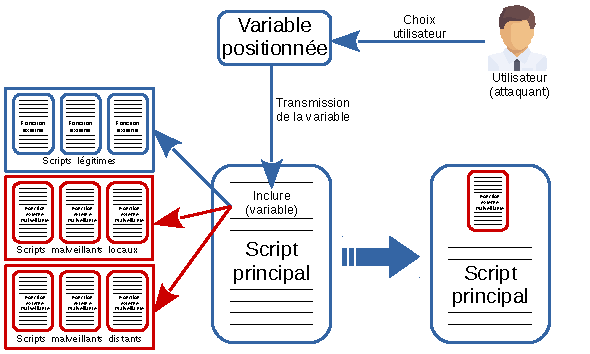
\includegraphics[scale=1.4]{images/include_hacked.pdf}

\caption{Vulnérabilité d'inclusion d'un fichier}

\end{center}
\end{figure}

On remarque dans le schéma \ref{inclusion_hacked} que dans le cas où un attaquant peut avoir accès à la variable permettant de sélectionner le script légitime, celui-ci peut en modifier le contenu de deux façons. On parle alors de Local File Inclusion (LFI) et de Remote File Inclusion (RFI).

\subsubsection{Local File Inclusion}

Une fois que l'attaquant est en capacité de modifier le contenu de la variable indiquant le nom du script à inclure, celui-ci peut y indiquer un chemin local (i.e. directement sur le serveur) vers un script contenant du code malveillant. Il peut s'agit d'un script que l'attaquant a au préalable placé sur le serveur ou d'un script déjà présent qui effectue des opérations pouvant porté atteinte à la disponibilité de la machine voire à l'intégrité ou la confidentialité des données.

\subsubsection{Remote File Inclusion}

L'attaquant peut également indiquer dans la variable un chemin distant (i.e. vers un autre serveur) pointant vers un script contenant du code malveillant. Cette technique a pour avantage de faciliter la gestion du contenu du script malveillant par l'attaquant qui peut y inclure toutes les fonctionnalités qu'il souhaite voire le faire évoluer en fonction de la réponse de la machine attaquée.\\

Dans les deux cas, les scripts malveillants sont recopiés au sein du code du script principal qui sera au final exécuté par le serveur. Cette vulnérabilité offre donc de vastes possibilités à un attaquant qui peut alors faire exécuter par un serveur n'importe quelles fonctionnalités qu'il souhaite.

\subsection{Exploitation de la vulnérabilité}

\subsection{Contre-mesure}

\section{File upload}

\subsection{Description de la vulnérabilité}

\subsection{Exploitation de la vulnérabilité}

\subsection{Contre-mesure}

\section{Insecure CAPTCHA}

\subsection{Description de la vulnérabilité}

\subsection{Exploitation de la vulnérabilité}

\subsection{Contre-mesure}








